\documentclass[12pt]{article}
\usepackage[english]{babel}
\usepackage{graphicx}
\usepackage[margin=3cm]{geometry}

\usepackage{amsmath, amssymb, amsthm}
\theoremstyle{plain}
\newtheorem{theorem}{Theorem}
\newtheorem{proposition}{Proposition}
\newtheorem{lemma}{Lemma}
\newtheorem{corollary}{Corollary}
\theoremstyle{remark}
\newtheorem{remark}{Remark}
\newtheorem{exercise}{Exercise}
\newtheorem{example}{Example}
\newtheorem{warning}{Warning}

\newcommand{\boR}{\mathbb{R}}
\newcommand{\boC}{\mathbb{C}}
\newcommand{\boE}{\mathbb{E}}

\usepackage{listings}
\usepackage{hyperref}
\usepackage{courier}

%\usepackage{layout}
\usepackage{xcolor}
\definecolor{commentgreen}{RGB}{2,112,10}
\definecolor{eminence}{RGB}{108,48,130}
\definecolor{weborange}{RGB}{255,165,0}
\definecolor{frenchplum}{RGB}{129,20,83}
\definecolor{lgrey}{RGB}{235,235,235}

\lstset{
  linewidth=17cm,
  %xleftmargin=0cm,
  %xrightmargin=-1cm,
}


\lstdefinestyle{C}{
  language=C,                     % choose the language of the code
  numbers=left,                   % where to put the line-numbers
  stepnumber=1,                   % the step between two line-numbers.        
  numbersep=10pt,                  % how far the line-numbers are from the code
  inputencoding=utf8,
  upquote=true,
  commentstyle=\color{commentgreen},
  keywordstyle=\color{eminence},
  stringstyle=\color{red},
  basicstyle=\footnotesize\ttfamily, % basic font setting
  emph={int,char,double,float,unsigned,void,bool},
  emphstyle={\color{blue}},
  showspaces=false,               % show spaces adding particular underscores
  showstringspaces=false,         % underline spaces within strings
  showtabs=false,                 % show tabs within strings adding particular underscores
  tabsize=8,                      % sets default tabsize to 2 spaces
  breaklines=false,                % sets automatic line breaking
  breakatwhitespace=true,         % sets if automatic breaks should only happen at whitespace
  title=\lstname,                 % show the filename of files included with \lstinputlisting;
  frame=tb,
  captionpos=tb,                  % sets the caption-position to bottom
  backgroundcolor=\color{lgrey},  % choose the background color. You must add \usepackage{color}
}

\lstdefinestyle{Python}{
  language=Python,                     % choose the language of the code
  numbers=left,                   % where to put the line-numbers
  stepnumber=1,                   % the step between two line-numbers.        
  numbersep=10pt,                  % how far the line-numbers are from the code
  inputencoding=utf8,
  upquote=true,
  commentstyle=\color{commentgreen},
  keywordstyle=\color{eminence},
  stringstyle=\color{red},
  basicstyle=\footnotesize\ttfamily, % basic font setting
  %emph={int,char,double,float,unsigned,void,bool},
  emphstyle={\color{blue}},
  showspaces=false,               % show spaces adding particular underscores
  showstringspaces=false,         % underline spaces within strings
  showtabs=false,                 % show tabs within strings adding particular underscores
  tabsize=4,                      % sets default tabsize to 2 spaces
  breaklines=false,                % sets automatic line breaking
  breakatwhitespace=true,         % sets if automatic breaks should only happen at whitespace
  title=\lstname,                 % show the filename of files included with \lstinputlisting;
  frame=tb,
  captionpos=tb,                  % sets the caption-position to bottom
  backgroundcolor=\color{lgrey},  % choose the background color. You must add \usepackage{color}
}

\lstdefinestyle{bash}{
	backgroundcolor=\color{lgrey},
	basicstyle=\color{black}\footnotesize\ttfamily\selectfont,
	breakatwhitespace=false,  
	breaklines=true,
	captionpos=b,
	commentstyle=\color{commentgreen},
	escapeinside={\%*}{*)},
	extendedchars=true,
	frame=none,
	keepspaces=true,
	keywordstyle=\color{green},
	%language=bash,
	morekeywords={@},
	numbers=none,
	showspaces=false,
	showstringspaces=false,
	showtabs=false,
	stepnumber=2,
	stringstyle=\color{weborange},
	tabsize=2
}

\usepackage{algorithm, algpseudocode, float}



\title{MU4MA016 course notes}
\author{Didier Smets}

\begin{document}

\maketitle

\noindent \underline{{\sc Week 1 : Sept. 5th 2024}}

\bigskip

The course being entitled {\bf Algorithms} and {\bf Data Structures} for {\bf
Computer programming}, in this introductory lecture we will briefly discuss each 
of these three words, trying to highlight by some simple examples the kind of
questions which will interest us in the following.

\section{Algorithm}

The following algorithm was originally described by Euclid in order to find
the greatest common divisor (gcd) between two positive integers $a$ and $b$.

\begin{algorithm}[H]
\caption{Euclid's algorithm (original version)}
\begin{algorithmic}
\Require $a, b$ are positive integers
\Function{gcd}{$a$, $b$}
\While{$a \neq b$}
\If{$a > b$}
\State $a \gets a - b$
\Else{}
\State $b \gets b - a$
\EndIf
\EndWhile
\State \Return a
\EndFunction
\end{algorithmic}
\end{algorithm}

The above description is called {\tt pseudo code}. It is intended to be read my
humans, and it must be unambiguous for humans. Instead, computer programs which
we will tackle later, are intended to be read by computers (compilers or
interpreters), which implies further restrictions on them (both syntaxic and
in terms of the operations available). 

Among the properties of algorithms, we will be particularly interested in the
following :
\begin{itemize}
\item Correctness : that is the least one should ask for, but it needs not be overlooked !
\item Complexity : both time and space complexity (to be explained below).
\item Ease of implementation : because in the end it will need to be turned
into a program.
\end{itemize}

\subsection*{Correctness}
In the case of Euclid's algorithm we could argue along
the following lines :
\begin{enumerate}
\item After each step of the while loop, $a$ and $b$ remain both
	positive\footnote{Note to french speaking students : in mathematical english
		{\bf positive} means ``strictement positif''; the french ``positif''
		is instead translated as {\bf non negative}.}
Indeed they must be different to enter the loop and the smaller is subtracted
from the larger. 
\item Because of the previous claim, the sum $a + b$ decreases strictly after
each step of the loop. In particular, there can be at most finitely many steps
of the loop and therefore the algorithm will always terminate.
\item Let $c$ be the actual greatest common divisor of $a$ and $b$. Then after
each step of the loop, $c$ is still a divisor of $a$ and $b$. Indeed, if a
number divides two other numbers, then it also divides their difference. Since
the algorithm eventually returns (the modified version of) $a$, let's call it
$d$, it follows that $c$ divides $d$.
\item We next claim that $d$ divides (the original values of) $a$ and $b$. To
prove this we argue as above, but backward. First, at the end of the while loop
we have $a = b = d$, and therefore $d$ divides both $a$ and $b$. Now if $d$
divides $a$ and $b$ after some (arbitrary) step of the loop, it also did at the
previous one. This is because if a number divides two other numbers, it also
divides their sum (and running a step backward correspond to changing one of
them to the sum of the two). 
\item In summary, we have shown on one hand that $c$ divides $d$ (in particular
$c \leq d$), and on the other hand that $d$ divides $a$
and $b$. By definition of $c$ being the greatest common divisor of $a$ and $b$,
it follows that $c = d$, which proves the correctness.
\end{enumerate} 

In many cases, proving algorithm correctness proceeds by showing that some form
of invariant is preserved during the process (especially when some loops are
involved). In the example above, the invariant was the divisibility by $c$.

\subsection*{Complexity}

As mentioned already, for all the algorithms we will study, we shall discuss both {\bf
time complexity} and {\bf space complexity}. These notions only make rigorous 
sense within a so-called {\it computation} and a {\it memory} model, but in short :
\begin{itemize}
\item The time complexity measures how much computations the algorithm
needs to perform in order to provide its result. Since the number may
depend on the input values, it is often useful to distinguish between
the worst case scenario and some form of average case.
\item The space complexity measures the amount of local storage required by
the algorithm in order to perform its computations, in addition to the storage
of its inputs.
\end{itemize}

In practice the two notions often pull in opposite directions, and the optimum 
is a matter of compromise.

\medskip

In the case of Euclid's algorithm, space complexity is trivial: no temporaries
are required since only updates of the original variables occur. Time complexity
(assuming that comparison and arithmetic operations can all be performed in
$O(1)$ time\footnote{As reasonable as it may look, in practice most
implementations would implicitly require that the input integers fit in some range
allowing them to be represented easily on the architecture, e.g. over 64bits, 
which by nature kills the whole meaning of $O()$ analysis, but that is what it
is...}) can easily be computed to be $O(\max(a, b))$, where the worst case
happens when one of the two values, say $b$, is $1$ (just think of the routing of the algorithm
in that case, leading to $a$ being decreased by $1$ at each step until it
reaches $1$). 

\medskip

The following variant is actually often called the Euclid algorithm too, 
although it was not presented by Euclid in this form.

\begin{algorithm}[H]
\caption{Euclid's algorithm (improved version)}
\begin{algorithmic}
\Require $a, b$ are positive integers
\Require $c$ a temporary storage for an integer
\Function{gcd}{$a$, $b$}
\While{$b \neq 0$}
\State $c \gets b$ 
\State $b \gets a \textrm{ modulo } b$
\State $a \gets c$
\EndWhile
\State \Return a
\EndFunction
\end{algorithmic}
\end{algorithm}

\noindent {\bf Exercise :} 
\begin{itemize}
\item Prove the correctness of this second version.
\item Prove that its time complexity is $O(\log(\max(a, b)))$.\\{\it Hint:
	proceed backward and compare the current values of $a$ and $b$ to the
		Fibonacci sequence defined by $F_0=0$, $F_1=1$ and $F_{k+2} =
		F_{k+1} + F_{k}$.}
\end{itemize}

In practical applications, a logarithmic complexity is a really strong 
and desirable one, in comparison e.g. here to the linear complexity of 
the original version. Even worse would be a quadratic, cubic, general polynomial
or even non polynomial (abbr. as NP) complexity.

\section{Data Structure}

Consider the following two variants of the birthday-matching problem (i.e.
determine if at least two among a class of students have the same anniversary
date, omitting year).

\begin{algorithm}[H]
\caption{Birthday match using sets}
\begin{algorithmic}
\Require As input, a set of students, called $class$
\Require As temporary storage, a set of students called $visited$
\State Initialize $visited$ as the empty set
\ForAll{student $a$ in $class$}
\ForAll{student $b$ in $visited$}
\If{$birthday\_match(a, b)$}
\State \Return true
\EndIf
\EndFor
\State Insert $a$ into $visited$
\EndFor
\State \Return false
\end{algorithmic}
\end{algorithm}

We have implicitly assumed here that we have a notion of {\it Set}, over which we can
{\it Iterate}, and which we can grow by make use of some {\it Insert}.

An {\bf Abstract Data Structure (ADT)} is an abstract description of 
\begin{enumerate}
\item What kind of data can be stored (possibly referring to other existing ADT)
\item What operations can be performed on these data
\end{enumerate}


In terms of time complexity, in worst case scenarios we will need to apply
$O(N^2)$ (where $N$ is the number of students in class) times the birthday match
check. We should also take into account the time complexity associated to the
{\it Iterate} (for all) and {\it Insert} functions. These later must either be
postulated (as we did for the arithmetic operations in Euclid's), or guaranteed 
by some implementation of a Concrete Data Structure within a computing and
memory model.

\medskip

In terms of space complexity, the set $visited$ may grow at most to a size of
$N$. With the same caution as above regarding theory vs implementation, we will say that 
the space complexity is therefore $O(N)$.


Note that whenever $N > 365$, the algorithm could exit early with {\it true}, by
an immediate application of the pigeon-hole principle\footnote{If there are more pigeons than
cages, at least two pigeons must share the same cage. In french: ``Principe des
tiroirs''.} Not only this underlines
the caution that should always accompany asymptotic analysis in finite
frameworks, but it also suggests a very different variant~: 

\begin{algorithm}[H]
\caption{Birthday match using an array}
\begin{algorithmic}
\Require As input, a set of students, called $class$
\Require As temporary storage, an array $A$ of 365 boolean
\State Initialize all entries of $A$ with false
\ForAll{student $s$ in $class$}
\State Let $k$ be the anniversary date of $s$ (view as an integer $1 \leq k \leq 365$)
\If{$A[k] = true$}
\State \Return true
\Else
\State $A[k] \gets true$
\EndIf
\EndFor
\State Return false
\end{algorithmic}
\end{algorithm}

The time complexity of this variant is now only $O(N)$ (with the same caution as
before), and the space complexity is fixed, independently of the size of the
class, therefore $O(1)$.

\medskip

\noindent{\bf Exercise : } Replace 365 by an integer $M$ (imagine we compare
some ID numbers instead of birthdays), and assume that both $M$ and $N$ get
large but also that $M \gg N$ (by this we mean that $M$ is much larger than $N$)
and that a spatial complexity of $O(M)$ is forbidden because it would be too
large in practice. Are we forced to resort to the first version of the
algorithm, or could do better ? ({\it Hint: hash tables and sorted trees are both in the
menu for later}).

\bigskip

The data structures that we shall go over in this course include : arrays,
stacks, queues, lists, hash tables, (binary search) trees, heaps and graphs.
Different implementations may use different concrete data structures to 
represent the same abstract data structure. The abstract notion of Set or of
Dictionary, is often implemented either via a hash table, or with some form
of tree. 

\section{Computer Programming}

We are not going to study computer programming per se\footnote{In particular this 
is not a course on the latest hype in C++ !}, but we are going to study how to 
efficiently implement (good) algorithms on computers, using specific languages.

As scientific programmers, there are essentially two choices, which differ by 
their strong points and limitations.
\begin{itemize}
\item Using a high level language, offering a number of high level native data
structures, and potentially also an interactive interpreter. This is the case
e.g. of Python and its CPython interpreter, or of Julia with its 
just-in-time (JIT) compiler. This is the easiest to start with, 
and it can be efficient too when appropriate libraries (coded in low level
languages) are available for the task of choice, like e.g. Numpy just to name
one. This is also a very good test bed for profiling a new algorithm on small
data sets, before turning to a lower level language for performance on large 
scale data sets.
\item Using a lower level language, giving a closer access to the hardware or
at least to the virtual memory, and which can be compiled into efficient machine
code due to compiler optimizations. This is the case e.g. of C/C++, and the
one we will use in this course.
\end{itemize}

The syntax and grammar of C will not be taught in class. There are very good
references online, C grammar is easy, and those who have never met with it 
will catch-up quickly in the first TP classes. From C++ (kind of a superset of
C) we will only ever borrow a few features that {\it may} sometimes be handy.

\medskip

Although lower level languages are said to be closer to the hardware, in
this course for the most we will only need to understand an take into
account the following. The storage memory is presented to us by the 
operating system (OS) as a large addressable 1D array, the so-called 
{\it virtual memory}, and
\begin{enumerate}
\item 
{\bf The access time needed to bring back some data from RAM to the CPU can
be much larger than the typical time needed by the CPU to perform some
		computation/instruction} (one
usually measures time in so-called CPU cycles). As of today, it can be by a 
factor 100x to 1000x, with respect e.g. to an arithmetic operation.
\item
In order to overcome this otherwise huge bottle-neck in computation, a number of 
physical levels of so-called caches are introduced in between the CPU and the RAM. 
You can think of these cache levels as smaller but faster access memories, and
there are strategies (independent of us) to decide what is kept in cache (I
like the analogy of RAM being the university library, the next level of cache 
is your home bookshelf, and the closest level of cache to CPU is your
nightstand). {\bf The
important thing to remember as a programmer, is that if some data is put into cache,  
then the ``nearby'' data (in the virtual memory 1D array) is brought at the same time, 
and therefore it will be readily available provided our successive accesses to memory 
are sufficiently local}. 
\end{enumerate}

This notion of {\it locality} is well understood (and can be experienced!) in the following
simple yet typical example of the computation of the product $A * B$ of two
matrices, say of size $N \times N.$

\medskip

Let's first implement it (in language C) in the way you were taught about the matrix
product in Math classes. Note first that the memory being a 1D array, matrices need to
be ``flattened'' to be recorded in memory. The so-called {\it row-major} convention, 
i.e. line after line, where the equivalent of what we write $A(i,j)$ in math is
accessed in $A[i * N + j]$, is the most popular in C language implementations. 
The other obvious alternative, the so-called {\it column-major} convention, was 
most popular in Fortran language. Which algorithm works best for a matrix
product is highly dependent of the choice of the convention, as we shall
experience ! In the sequel we choose the {\it row-major} standard C
convention. Note also that in C, indices for array indexing start at $zero$,
not at $1$ as we usually do in math, this eases address computations.  

\begin{lstlisting}[style=C]
void matrix_product1(float C[], const float A[], const float B[], int N)
{
	for (int i = 0; i < N; ++i) {
		for (int j = 0; j < N; j++) {
			/* Compute C_{i,j} */
			C[i * N + j] = 0;
			for (int k = 0; k < N; k++) {
				C[i * N + j] += A[i * N + k] * B[k * N + j];
			}
		}
	}	
}
\end{lstlisting}

When the loop counters $i$, $j$ or $k$ are incremented, the data locations involved in the
actual product computation on line 8 vary differently. An increment of $i$ leads
to a jump of $N$ (times the size of a float, not repeated later) in memory for $C$ and $A$. An
increment of $k$ introduces a jump of $N$ in the memory location for $B$, and finally an
increment of $j$ only induces increments of one (i.e. no jump, i.e. local). 
By far the most problematic of all these is the jump of $N$ introduced by an
increment of $k$ : indeed it arises at every of the $N^3$ steps of the three
nested loops. The increment of $i$ causes the same jump of $N$, but it only
occurs $N$ out of the $N^3$ steps, which is negligible in proportion. This
implementation, at least for large values of $N$, will therefore likely 
be memory bottlenecked.

\medskip

Instead, let us propose the following alternative obtained for the most 
by a permutation of the loops in $j$ and $k$ :
\begin{lstlisting}[style=C]
void matrix_product2(float C[], const float A[], const float B[], int N)
{
	for (int i = 0; i < N; ++i) {
		/* Zero initialize C */
		for (int j = 0; j < N; j++) {
			C[i * N + j] = 0;
		}
		for (int k = 0; k < N; k++) {
			for (int j = 0; j < N; j++) {
				/* Update C_{i,j} */
				C[i * N + j] += A[i * N + k] * B[k * N + j];
			}
		}
	}	
}
\end{lstlisting}

\noindent{\bf Exercise :} First convince yourself that this second version also
actually computes the product of $A$ and $B$ ! Then analyze the memory accesses
as above, and observe that the non local jumps only occur now $N^2$ out of $N^3$
times, which is negligible in proportion if $N$ is large, and therefore should 
better avoid the memory latency problem.

\medskip

\noindent{\bf Exercise :} Check it in practice by testing e.g. with $N = 1000$, 
after you will be familiar with C and gcc in the first TP classes. 
In these tests, try both the compiler optimization {\tt -O0} (i.e. no
optimization) and {\tt -O3} (most optimizations).

\medskip

\noindent{\bf Proposed solution}
Here is a proposed test implementation, that will serve for those of you
discovering C. Reproduce and test on your own !

\lstinputlisting[style=C]{data/matrix_multiplication_test.c}

We then compile it (first with zero optimization) :

\begin{lstlisting}[style=bash]
@: gcc -Wall matrix_multiplication_test.c -o matrix_multiplication_test
\end{lstlisting}

and test it

\begin{lstlisting}[style=bash]
@: ./matrix_multiplication_test 1000
Timer Algo 1: 4.159 s
Sum of C : 250005104.000000
Timer Algo 2: 3.229 s
Sum of C : 250005104.000000
\end{lstlisting}

We can observe a modest difference but not great. Let's introduce compiler
optimization (level 3 = all).

\begin{lstlisting}[style=bash]
@: gcc -Wall -O3 matrix_multiplication_test.c -o matrix_multiplication_test
@: ./matrix_multiplication_test 1000
Timer Algo 1: 1.031 s
Sum of C : 250005104.000000
Timer Algo 2: 141.192 ms
Sum of C : 250005104.000000
\end{lstlisting}

First as you can see the -O3 flag implied a great speed-up, but more importantly 
the {\tt\_v2} version of the algorithm also now runs one order of magnitude faster than 
the {\tt\_v1} one !

\medskip

\begin{remark} Although the matrices $A$ and $B$ 
were filled with random real numbers between 0 and 1, the sum of 
the coefficients of $C$ seems to be an integer. How is that possible ?!\\ 
The (pseudo)-random values stored in $A_{ij}$ and $B_{jk}$  are supposed
to model a uniform distribution on $[0,1]$, therefore
$$
\boE(sum(C)) = \sum_{i,j,k = 1}^N \boE(A_{ij}B_{jk}) =  \sum_{i,j,k = 1}^N
\boE(A_{ij}) \boE(B_{jk}) = \frac{N^3}{4},
$$
where we have used that $A_{ij}$ and $B_{jk}$ are independent (they are
different samplings of the random variable) and $\boE(A_{ij}) = \boE(B_{jk}) =
\frac{1}{2}$ for a uniform variable over $[0,1]$. For $N = 1000$, we expect therefore
that $\boE(sum(C)) = 2.5e8$, which indeed is an integer. But the error itself,
in the example sampling above $5104$, has no reason to be an integer. This is
not at all related to the maths, but instead to the way real numbers (here 32
bits floating points) are stored in a computer, we will discuss that into more
details later. 
Not all real numbers are represented (there would be infinitely
many of them!), and it happens that within 32bits floats the closest float to
$2.5e8$ is $2.5e8 + 1.$ If you take $N = 100$ instead, you'll start
observing fractional parts in the answer.
\end{remark}

\begin{exercise} Compute that
$$
\boE(sum(C)^2) = \frac{1}{16}N^6 + \frac{1}{24}N^4 + \frac{1}{36}N^3
$$
and therefore that 
$$
\Sigma(sum(C)) = \sqrt{Var(sum(C))} = \sqrt{N^4/24 + N^3/3} \simeq 0.2 N^2
\text{ for N large}.
$$
Run the test above multiple times, of with different values of $N$, and
observe/check then that the deviation to the expected value is indeed 
of the order of the standard deviation $\Sigma(sum(C)) \simeq 0.2 N^2$.\\
{\it Hint : while evaluating termes of the form
$\boE(A_{ij}B_{jk}A_{i'j'}B_{j'k'})$, distinguish between the three cases : 
a) $(i,j,k) = (i',j',k')$, b) $(i,j) = (i',j')$ or $(j,k)=(j',k')$ but $(i,j,k)
\neq (i',j',k')$, and finally c) $(i,j) \neq (i',j')$ and $(j,k) \neq (j',k')$. 
Recall also that whenever $X$ is uniform over $[0,1]$, $\boE(X^2) = 
\int_0^1 x^2\, dx = \frac{1}{3}$.} 
\end{exercise}

\medskip

Finally, let us compare our code performance with respect to Python, either
using pure Python loops or using available scientific libraries, the most
famous being Numpy (it is internally coded in C!).

\lstinputlisting[style=Python]{data/matrix_multiplication_test.py}

We obtain :  

\begin{lstlisting}[style=bash]
@: python3 matrix_multiplication_test.py
Pure Python for N =   10 : 0.00117s
Pure Python for N =   20 : 0.00923s
Pure Python for N =   50 : 0.07167s
Pure Python for N =  100 : 0.52314s
Pure Python for N =  200 : 4.19137s
Using Numpy for N = 1000 : 0.00737s
Using Numpy for N = 2000 : 0.04697s
Using Numpy for N = 4000 : 0.35011s
\end{lstlisting}

A number of remarks are in order :
\begin{enumerate}
\item
For both algorithm, we can observe the expected behaviour of a cubic time
complexity. Note that algorithm with a lower power of $N$ do exist (see e.g. 
this \href{https://en.wikipedia.org/wiki/Computational_complexity_of_matrix_multiplication}{Wiki link}),
but they are complex to implement and often come with large pre-factor
constants. The most well-known is Strassen's algorithm, at $O(N^{\log_2(7)})
\simeq O(N^{2.8})$, but the present state of the art is $O(N^{2.37})$. Clearly 
any algorithm must be at least $O(N^2)$ (indeed at least the $N^2$ entries of
$C$ must be filled!), at least for a sequential algorithm, but it is open if 
one could go as low as $O(N^2)$.
\item
There is a {\bf huge} difference between the timings in pure Python and using
Numpy, more than three orders of magnitude. As a matter of fact, for pure Python I 
had to limit $N$ to a smaller value than a few hundreds in order to keep the script run 
time under control.
\item 
For $N = 1000$, Numpy is still 20 times faster that our current best
implementation in \tt{\_v2} !
\end{enumerate}

What can/should we do to improve our code to state of the art performance then ?

There are easy improvements :
\begin{enumerate}
\item Allow the compiler to use the whole set of CPU instructions for the computer
with are running on (this can be an issue if we wish to distribute our program to
machines which would not have all this set) The gcc option is {\tt -march =
native}. A safer yet usually as effective solution is to require a common vector
instruction set, like the MMX or AVX. We shall use the {\tt -mavx} gcc switch.
\item Modify our C code by adding the {\it restrict} keyword to the output array
pointer C of our matrix\_product functions. This tells the compiler that the place where
we write $C$ does not overlap (one says ``aliases with'') the one of $A$ and or
$B$, and avoids unnecessary copies. 
\item Modify our C code by forcing a 256 bits alignment for our
memory allocations of $A, B$ and $C$. This can improve the use of vector
instructions by the compiler (see 1) here above). To do so, we replace 
{\tt malloc} by {\tt aligned\_alloc}.
\end{enumerate}

\begin{lstlisting}[style=C]
void matrix_product_v2(float *__restrict C, const float *A, 
						const float *B, int N) {
[...]
}

[...]
	float *A = (float *)aligned_malloc(32, N * N * sizeof(float));
	float *B = (float *)aligned_malloc(32, N * N * sizeof(float));
	float *C = (float *)aligned_malloc(32, N * N * sizeof(float));
[...]
\end{lstlisting}
With these and the avx switch we obtain:
\begin{lstlisting}[style=bash]
@: gcc -Wall -O3 -mavx matrix_multiplication_test.c -o matrix_multiplication_test
@: ./matrix_multiplication_test 1000
Timer Algo 1: 1.042 s
Sum of C : 250279296.000000
Timer Algo 2: 69.523 ms
Sum of C : 250279296.000000
\end{lstlisting}
We have improved from $140ms$ to $70ms$, that is a factor 2, not bad ! Be we
ares still missing a factor almost 10. Let us observe the Operating System 
Monitor, first during our own implementation : 
\begin{center}
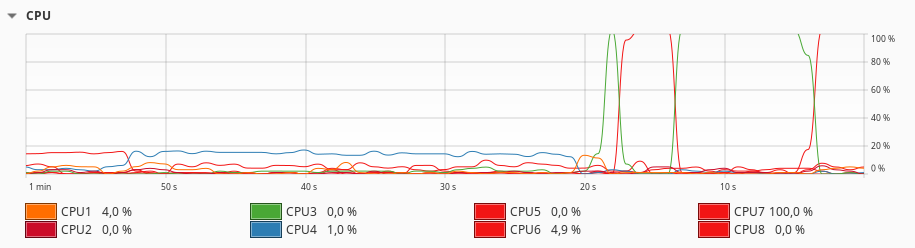
\includegraphics[width=15cm]{data/mat_mult_one_core.png}
\end{center}
and then during Numpy's implementation\footnote{In both cases, we have increased
$N$ so has to have time to take a screenshot !} 
\begin{center}
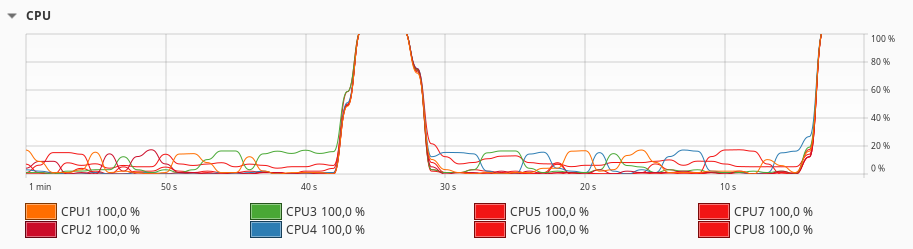
\includegraphics[width=15cm]{data/mat_mult_all_core.png}
\end{center}

The road-map is clear : our code is sequential, it uses just one CPU core, while
Numpy is making use of parallelism to use all the available 4 cores / 8 threads
in my (modest) computer ! 

\medskip

Numpy's (quite complex) source code can be browsed on Github 
\href{https://github.com/numpy/numpy/tree/main}{here}. One C source
file for (one of the possible versions of) matrix multiplication is
\href{https://github.com/numpy/numpy/blob/main/numpy/_core/src/umath/matmul.c.src}{this
one}. It has many includes and internal preprocessor macros making it difficult 
to read though, you may even have difficulties to recognize a valid C code.   

\medskip

Turning our matrix multiplication code into a parallel algorithm is one of the
very nice projects that you could implement for this course, especially for
those of you that are in the HPC program. Either making use of
CPU parallelism (using e.g. {\tt OpenMP} or better the lower level {\tt
pthread}), or even going to the GPU if one is 
available on your computer (using e.g. {\tt OpenCL}, {\tt OpenGL/Vulkan} 
compute shaders, or the proprietary {\tt CUDA}).

\medskip

In a broader perspective, parallelization of algorithms in many different areas
of Math/CS has been a very hot topic in recent years. This yields challenges both at the
algorithmic level, and at the implementation level. They require specific courses 
and we shall not dive too deeply into it, yet they all build upon the concepts
we shall develop in this course.

\end{document}
